\documentclass[12pt]{article}
\usepackage{fullpage}
\usepackage{subcaption,amsmath,amssymb,mathtools,xparse,graphicx,float,datetime,color,array,graphics,enumerate,tikz,pgfplots,xcolor}
\usepgfplotslibrary{statistics}
\pagestyle{empty}
\newcommand{\D}{\displaystyle}
\setlength{\textheight}{9in} \setlength{\headheight}{.2in}
\setlength{\headsep}{0in} \setlength{\topmargin}{0in}
\begin{document}
\begin{center}
CSCI 6100 Machine Learning From Data\\
Fall 2018\\
\end{center}
\begin{center}
HOMEWORK 9\\
Daniel Southwick\\
661542908\\
southd@rpi.edu
\end{center}
\vspace{.1in}

\noindent {\bf 1. 8th order Polynomial Feature Transform} \\\\
\indent For a $k$th polynomial feature transform, the number of features is $1 + 2 + 3 + ... + (k+1)$. So for an 8th order Polynomial Feature Transform, the number of feature is $1 + 2 + 3 + 4 + 5 + 6 + 7 + 8 = 45$. So $Z \in \mathbb{R}^{300 \times 45}$. \\

\noindent {\bf 2. Overfitting} \\\\
\indent With $\lambda = 0$, the algorithm overfitted the data, the boundary matches the training data too well and definitely has a large generalization error.
\begin{figure}[H]
  \centering
  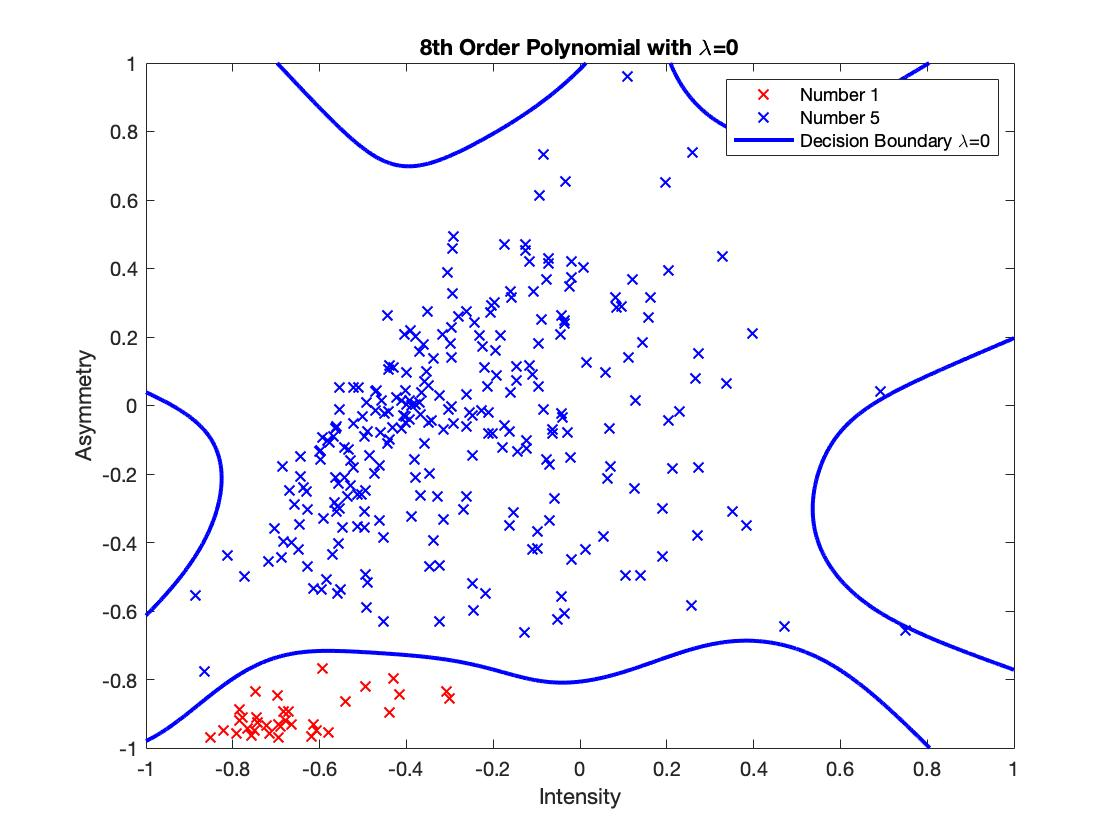
\includegraphics[scale = 0.3]{1.jpg}
  \caption{Decision Boundary with $\lambda = 0$}
  \label{fig:1}
\end{figure}

\newpage
\noindent {\bf 3. Regularization} \\\\
\indent Now, With $\lambda = 2$ regularization, the algorithm seems like it under fitted the data.
\begin{figure}[H]
  \centering
  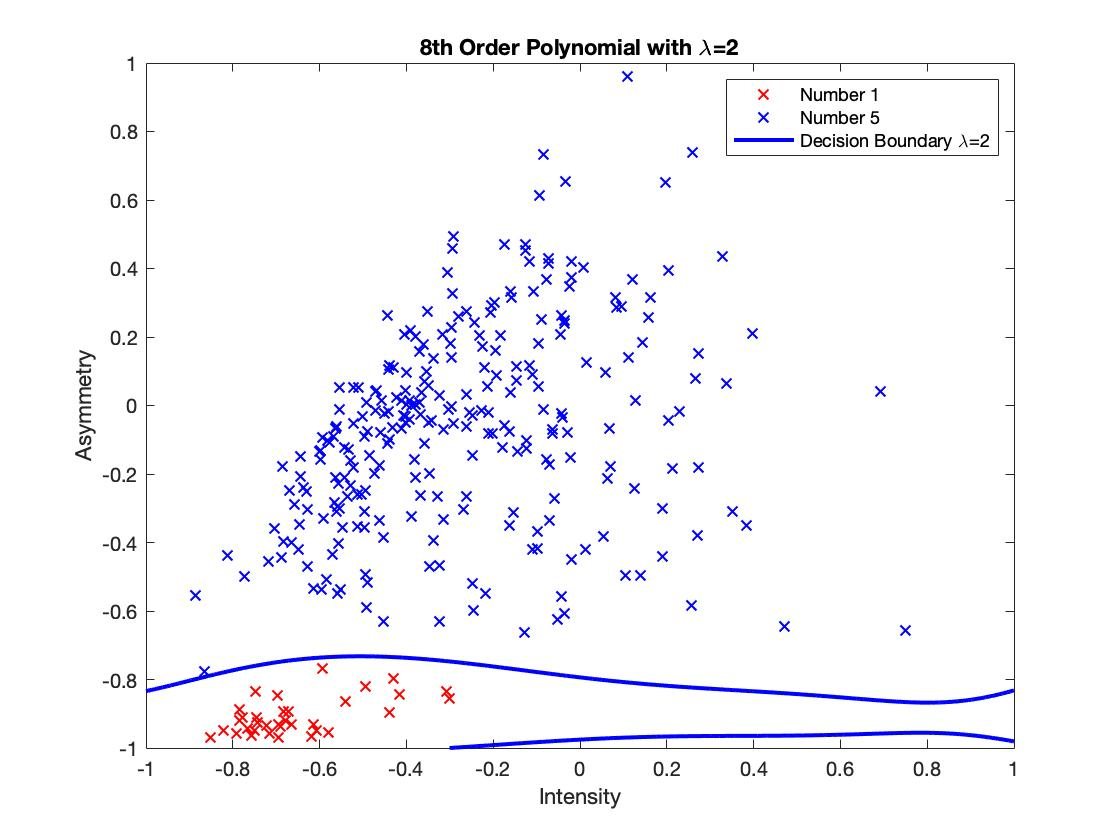
\includegraphics[scale = 0.3]{2.jpg}
  \caption{Decision Boundary with $\lambda = 2$}
  \label{fig:2}
\end{figure}

\noindent {\bf 4. Cross Validation} \\\\
\indent The cross validation can be estimated as:
\begin{align*} \displaystyle
H(\lambda) &= Z(Z^TZ + \lambda I)^{-1}Z^T \\
\hat{y} &= H(\lambda)y \\
E_{cv} &= \frac{1}{N}\sum_{i = 1}^{N}(\frac{\hat{y_n} - y_n}{1 - H_{nn}(\lambda)})^2
\end{align*}
We change the value of $\lambda$ and plotted the cross validation error:
\begin{figure}[H]
  \centering
  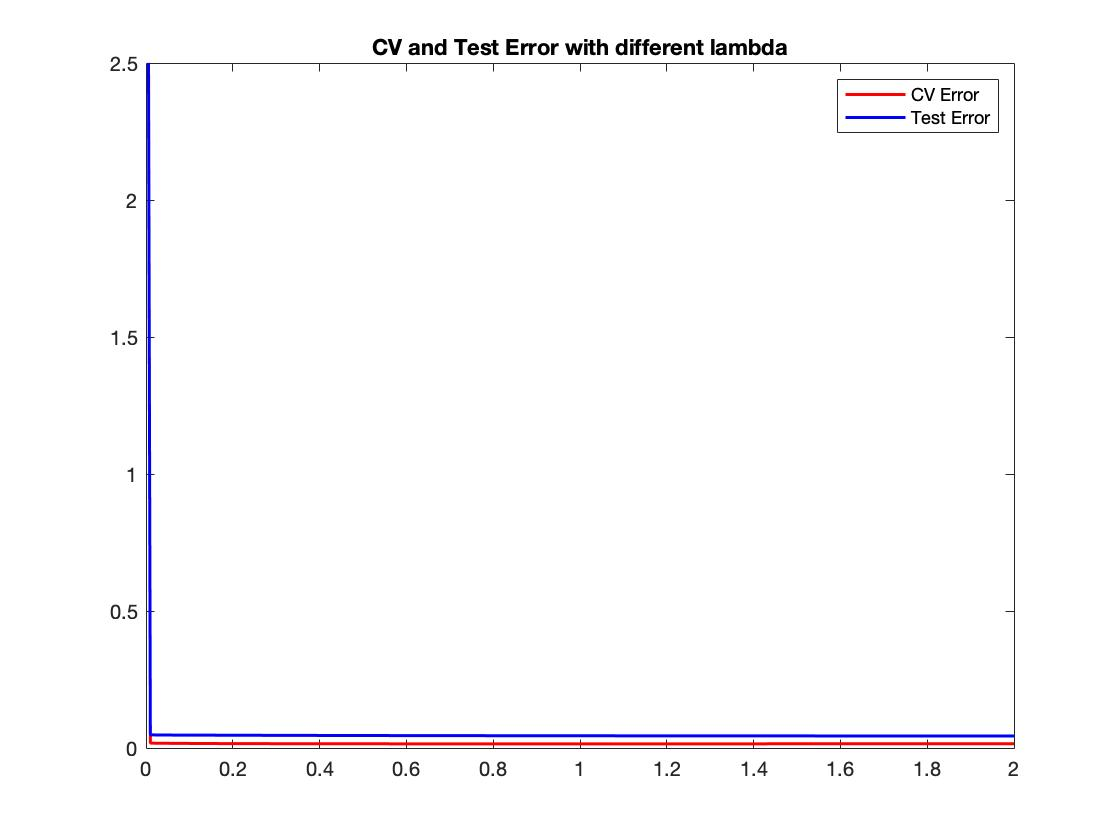
\includegraphics[scale = 0.25]{4.jpg}
  \caption{CV and Test Error for various $\lambda$}
  \label{fig:4}
\end{figure}
\indent $E_{cv}$ is always smaller than $E_{test}$, but it has the same trend as $E_{test}$, this means it reflects the changes of $E_{test}$\\

\noindent {\bf 5. Pick $\lambda^*$} \\\\
\indent Now, we let $\lambda = \lambda^*$, which is the smallest $E_{cv}$ corresponding $\lambda$, it is found to be $0.9$. and using the same method as $2$ and $3$, we retain the result as follows:
\begin{figure}[H]
  \centering
  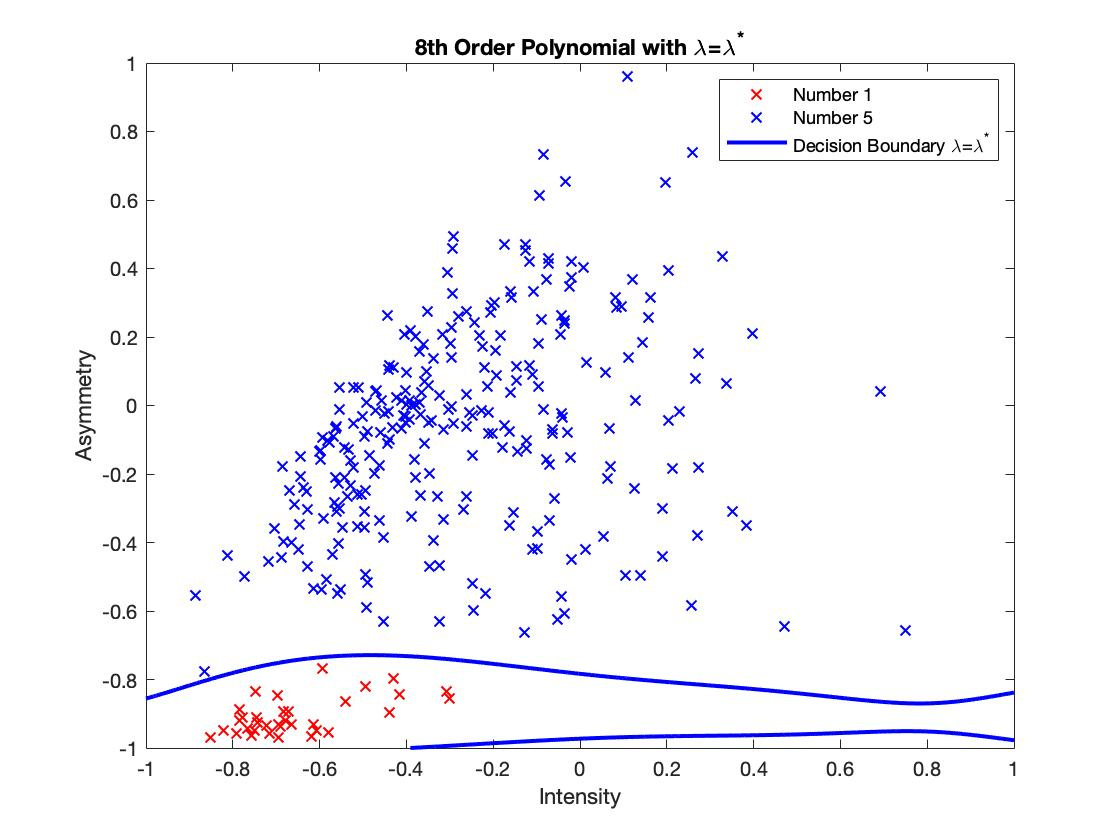
\includegraphics[scale = 0.3]{3.jpg}
  \caption{Decision Boundary with $\lambda = \lambda^*$}
  \label{fig:3}
\end{figure}

\newpage
\noindent {\bf 6. $E_{out}$ Estimation} \\\\
\indent $\lambda^* = 0.9$ and there are $8998$ data points within the test data and there are total of 109 points that got misclassified, and we set the tolerance to $\delta = 0.05$ so:
\begin{align*} \displaystyle
	E_{test} &= \frac{1}{N}\sum_{i = 1}^{N} 1_{sign(\hat{y_i} \neq y_i)} = 0.048\\
	E_{out}(g) &\leq E_{test}(g) + \sqrt{\frac{1}{2N}\ln \frac{2M}{\delta}} \\
	&\leq \frac{109}{8998}+ \sqrt{\frac{1}{2\times8998}\ln \frac{2\times1}{0.05}} \\
	&\leq 0.0118 + 0.0143\\
	E_{out}(g) &\leq 0.0261
\end{align*}
Therefore we have 95\% confidence to say $E_{out}$ is less than 0.0261\\\\

\noindent {\bf 7. $E_{cv}$ Biasity} \\\\
\indent $E_{cv}(\lambda^*)$ is not an unbiased estimate of $E_{test}( {w}_{reg}(\lambda^*))$. $E_{test}$ is the error from applying the hypothesis $g$ on the test dataset. While $E_{cv}$ is obtained with $g^-$, learned from $N-1$ data from the training dataset, since the $\lambda^*$ is selected based on the $E_{cv}$, thus $E_{cv}(\lambda^*)$ is not an unbiased estimate of $E_{test}( {w}_{reg}(\lambda^*))$.\\\\

\noindent {\bf 8. Data Snooping} \\\\
\indent $E_{test}( {w}_{reg}(\lambda^*))$ is not an unbiased estimate of $E_{out}( {w}_{reg}(\lambda^*))$. Since it chosen from the data set which was first split into training and testing dataset. $\lambda^*$ is selected from the training set and  $E_{test}( {w}_{reg}(\lambda^*))$ is computed after $\lambda^*$ is computed thus data snooping occurs. To fix it, we should use separate data set while doing validation, let it be fixed instead of random generated in this problem.


\end{document}

